\section{IBM Rational DOORS}
\label{chap:DOORS}

Das Anforderungsmanagement-Tool \ac*{DOORS} ist ein plattformübergreifendes und unternehmensweites Tool und wird
zur Erfassung, Verknüpfung, Verfolgung, Analyse und Verwaltung von Anforderungen genutzt. \acs{DOORS} ist ein Akronym,
das für Dynamic Object-Oriented Requirements System steht. Alle Anforderungen und weitere Informationen werden in einer zentralen Datenbank
gespeichert. Innerhalb der Datenbank werden die Informationen in Modulen gespeichert. Diese Module können mithilfe von Ordnern und Projekten
organisiert werden. Ordner sind vergleichbar mit den Ordnern z.B. im Windows Explorer und können andere Ordner, Projekte oder Module
beinhalten. Ein Projekt hingegen ist ein spezieller Ordner, der alle Daten für ein entsprechendes Projekt beinhaltet. Sowohl für 
Ordner als auch für Projekte können die Zugriffsrechte indiviuell eingestellt werden \cite[S.173]{DOORS}. Dabei existieren die Optionen
read, modify, create, delete und administer (RMCDA). 


\subsection{Module}

Es existieren zwei verschiedene Arten von Modulen im Anforderungsmanagement-Tool \acs{DOORS}. Module, die die eigentlichen Anforderungen
beinhalten, werden Formal Module genannt. Abbildung \ref*{fig:Modul Doors} zeigt ein Beispiel für so ein Modul. Zu erkennen ist dort
ein geöffnetes Formal Module. Auf der linken Seite ist ein Explorer zu sehen, auf der rechten Seite die eigentlichen Inhalte des Moduls.
Durch den Explorer auf der linken Seite, der in einer Baumstruktur organisiert ist, wird es dem User ermöglicht leicht zu einer bestimmten
Stelle im Modul zu navigieren. Die einzelnen Sektionen können dabei auf- und zugeklappt werden \cite[S.176]{DOORS}. Die Daten auf der 
rechten Seite sind tabellarisch angeordnet. Die Spalten stellen dabei die einzelnen Attribute des Moduls dar, während die Zeilen die 
Objekte darstellen. 

Neben den Formal Modules existieren auch die Link Modules. In diesen werden Informationen über die Beziehungen zwischen einzelnen Objekten
gespeichert.

\begin{figure}[h]
    \centering
    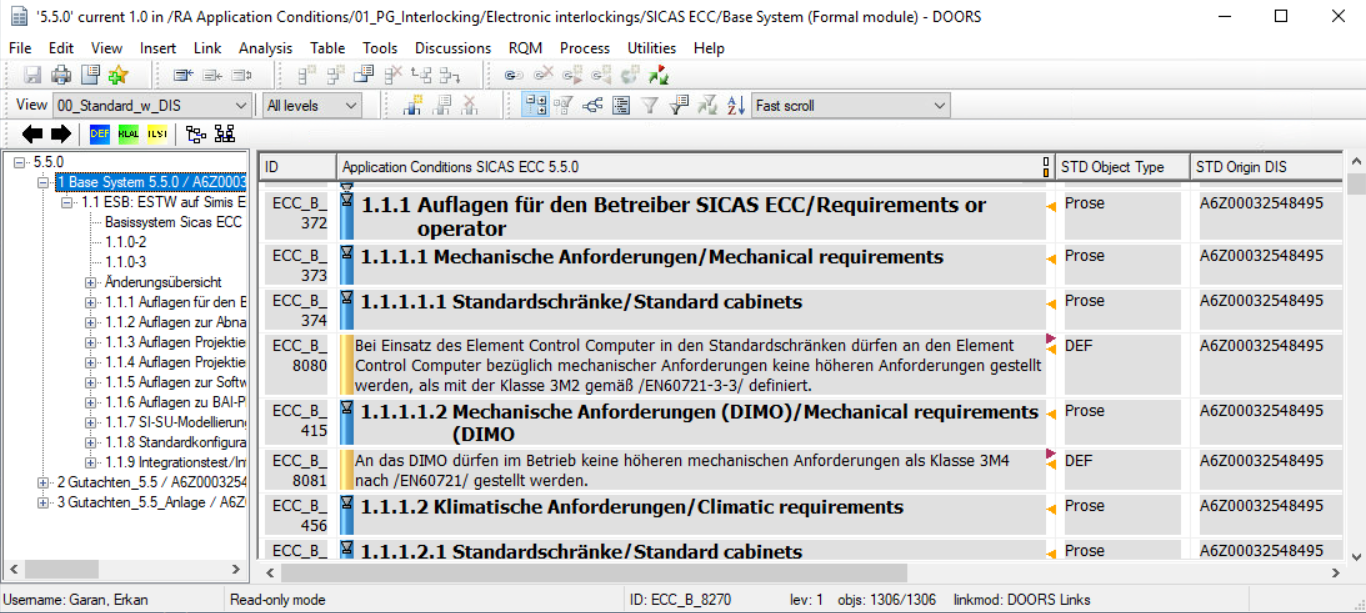
\includegraphics[width = \textwidth]{abbildungen/Modul in Doors.PNG}
    \caption{Geöffnetes Modul in \acs{DOORS}}
    \label{fig:Modul Doors}
\end{figure}


\subsection{Objekte und Attribute}
Innerhalb eines Moduls werden die Daten in Objekten gespeichert.
\subsection{Baseline}

\subsection{Links}

\subsection{DXL}

\ac*{DXL} ist eine Skript-Sprache, die speziell für das Anforderungsmanagement-Tool \acs{DOORS} entwickelt wurde. Durch diese Skript-Sprache
besteht die Möglichkeit die grafische Benutzeroberfläche von \acs{DOORS} um neue entwickelte Anwendungen zu
erweitern. Von der Syntax ähnelt die Sprache den Programmiersprachen C und C++ \cite[S.1]{DXL}. Zudem können Skripte geschrieben werden,
die als Batch-Script ausgeführt werden können. Diese Skripte bieten neben der grafischen Benutzeroberfläche eine weitere Möglichkeit, 
um mit \acs{DOORS} zu arbeiten. 
